\documentclass[11pt]{article}
\usepackage[a4paper,margin=25mm]{geometry}
\usepackage{amsmath,graphicx,booktabs,hyperref}
\title{Analytic verification of TensorFVM incompressible finite-volume solvers}
\author{Author details to be supplied}
\date{}
\begin{document}\maketitle
\begin{abstract}
A shared benchmark workflow evaluates plane Poiseuille flow and a periodic Taylor--Green vortex using raw numerical fields, declared relative error gates below 3 percent, refinement studies and independent replay. Negative controls are retained. These results establish bounded analytic verification, not engineering icebreaking qualification.
\end{abstract}
\section{Problem formulation}
For constant density, $\nabla\cdot\mathbf u=0$ and
$\rho(\partial_t\mathbf u+\nabla\cdot(\mathbf u\otimes\mathbf u))=-\nabla p+\nabla\cdot[\mu(\nabla\mathbf u+\nabla\mathbf u^T)]$.
The channel has $L=0.12$ m, $H=0.02$ m, $\rho=1000$ kg/m$^3$, $\nu=10^{-5}$ m$^2$/s and $U_b=5\times10^{-4}$ m/s. Uniform inlet and no-slip walls produce a developing entrance. Analytic comparison is restricted to $3H\leq x\leq5H$:
$u=6U_b(y/H)(1-y/H)$, $dp/dx=-12\mu U_b/H^2$, $|\tau_w|=6\mu U_b/H$.
Pressure curves are mean aligned only in this window.
The vortex has $[0,2\pi]^3$ m periodic boundaries, $\rho=1$, $\mu=0.1$, and
$u=\sin x\cos y e^{-2\nu t}$, $v=-\cos x\sin y e^{-2\nu t}$, $w=0$,
$p=\rho(\cos2x+\cos2y)e^{-4\nu t}/4$.
Velocity is sampled at its actual faces at $t=0.5$ s; pressure at cell centers and the last midpoint $t-\Delta t/2$, with zero mean.
\section{Methods and reproducibility}
Channel grids are $36\times12$, $72\times24$, $144\times48$, using staggered SIMPLE with $10^{-6}$ residual tolerance.
Periodic MAC uses compatible FFT projection, full symmetric stress and implicit midpoint. Spatial grids are $32^2$, $48^2$, $64^2$ with four z layers and $\Delta t=0.0125$ s. Temporal steps are $0.1$, $0.05$, $0.025$ s on $32^2\times4$.
Relative errors use global L2 or reference-peak Linf normalization. Time-order analysis uses the exact fixed-grid discrete eigenmode decay to isolate temporal error. Detailed metrics, clocks, source hashes, environment and raw fields accompany this manuscript.
\section{Results}
\resizebox{\linewidth}{!}{\begin{tabular}{llllrrl}\toprule
Case & Study & Grid & $\Delta t$ & $u$ L2 (\%) & $p$ metric (\%) & Gate\\\midrule
poiseuille & spatial & 36x12 & -- & 0.63436 & 1.36985 & PASS \\
poiseuille & spatial & 72x24 & -- & 0.16197 & 0.34402 & PASS \\
poiseuille & spatial & 144x48 & -- & 0.04285 & 0.07836 & PASS \\
taylor-green & spatial & 32x32x4 & 0.0125 & 0.03209 & 0.89781 & PASS \\
taylor-green & spatial & 48x48x4 & 0.0125 & 0.01427 & 0.39954 & PASS \\
taylor-green & spatial & 64x64x4 & 0.0125 & 0.00802 & 0.22480 & PASS \\
taylor-green & temporal & 32x32x4 & 0.1 & 0.03176 & 0.89426 & PASS \\
taylor-green & temporal & 32x32x4 & 0.05 & 0.03201 & 0.89803 & PASS \\
taylor-green & temporal & 32x32x4 & 0.025 & 0.03207 & 0.89817 & PASS \\
poiseuille & negative-control & 36x12 & -- & 25.35620 & 74.13972 & FAIL \\
taylor-green & negative-control & 16x16x4 & 0.0125 & 0.12793 & 3.56268 & FAIL \\
taylor-green-lbm & comparison & 32x32 & 0.00561798 & 0.63348 & 0.86173 & PASS \\
taylor-green-lbm & comparison & 64x64 & 0.00282486 & 0.15207 & 0.81428 & PASS \\
taylor-green-lbm & comparison & 32x32 & 0.00282486 & 0.64003 & 1.68311 & PASS \\
\bottomrule\end{tabular}}
\begin{figure}[htbp]\centering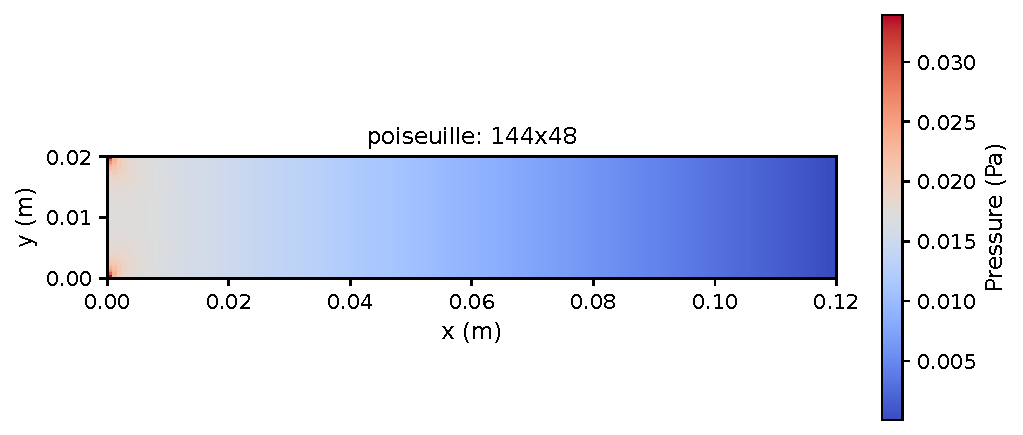
\includegraphics[width=0.9\linewidth]{channel-48/figures/pressure.pdf}\caption{poiseuille: pressure. Actual computed fields, SI units; comparison uses the documented reference region, gauge and time.}\end{figure}
\begin{figure}[htbp]\centering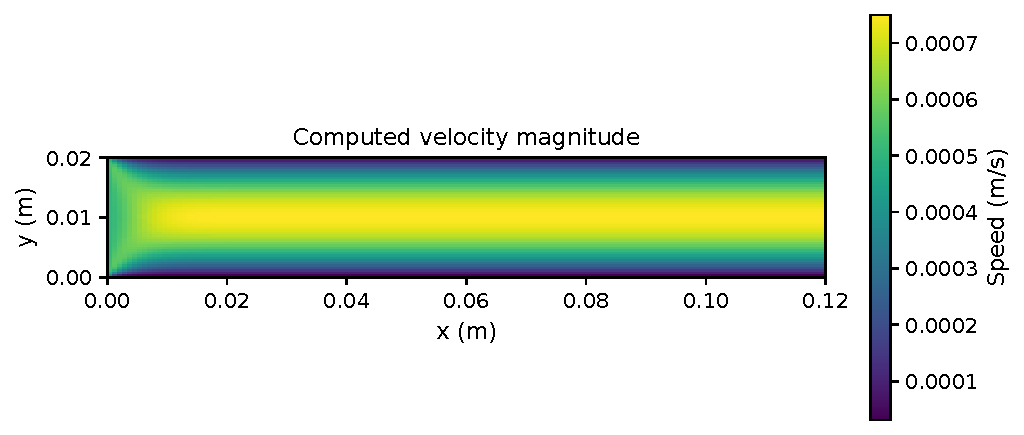
\includegraphics[width=0.9\linewidth]{channel-48/figures/speed.pdf}\caption{poiseuille: speed. Actual computed fields, SI units; comparison uses the documented reference region, gauge and time.}\end{figure}
\begin{figure}[htbp]\centering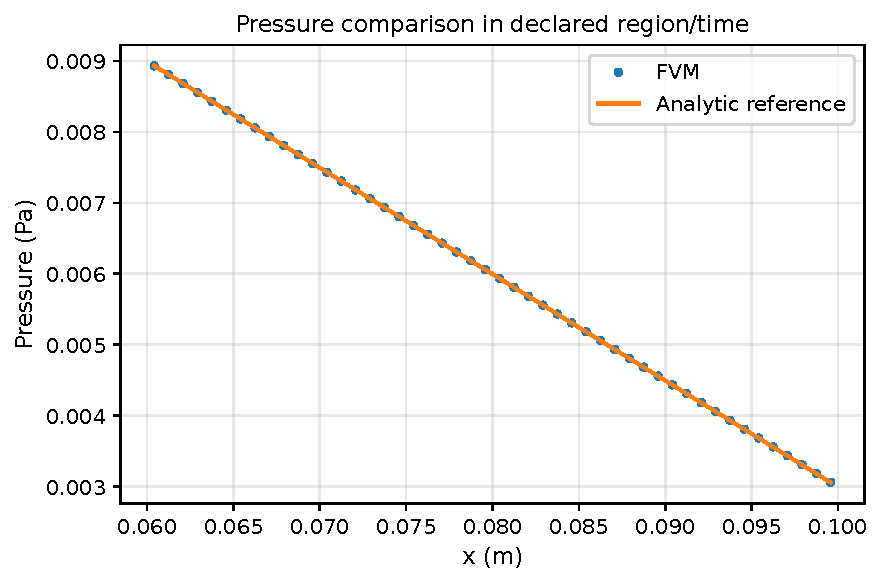
\includegraphics[width=0.9\linewidth]{channel-48/figures/pressure-curve.pdf}\caption{poiseuille: pressure-curve. Actual computed fields, SI units; comparison uses the documented reference region, gauge and time.}\end{figure}
\begin{figure}[htbp]\centering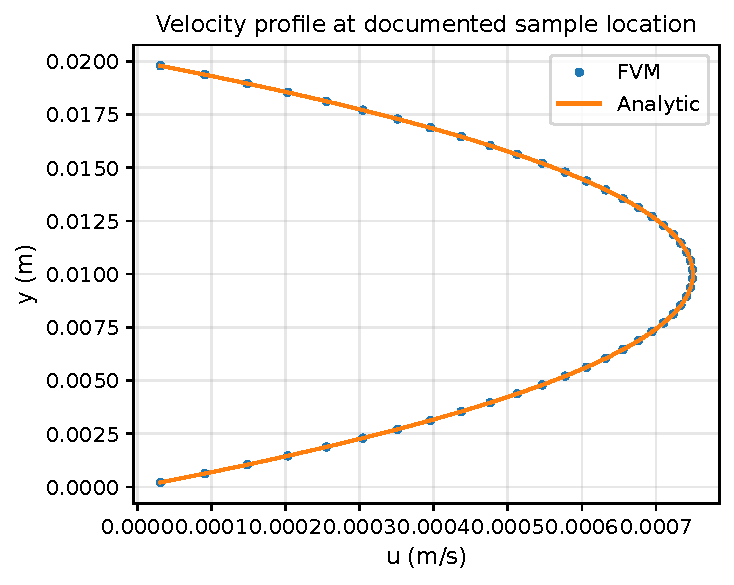
\includegraphics[width=0.9\linewidth]{channel-48/figures/velocity-profile.pdf}\caption{poiseuille: velocity-profile. Actual computed fields, SI units; comparison uses the documented reference region, gauge and time.}\end{figure}
\begin{figure}[htbp]\centering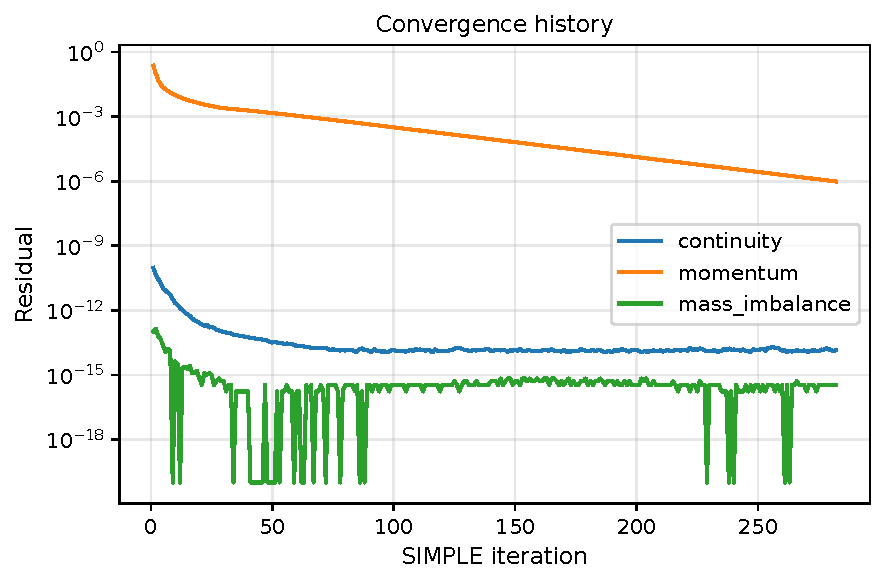
\includegraphics[width=0.9\linewidth]{channel-48/figures/history.pdf}\caption{poiseuille: history. Actual computed fields, SI units; comparison uses the documented reference region, gauge and time.}\end{figure}
\begin{figure}[htbp]\centering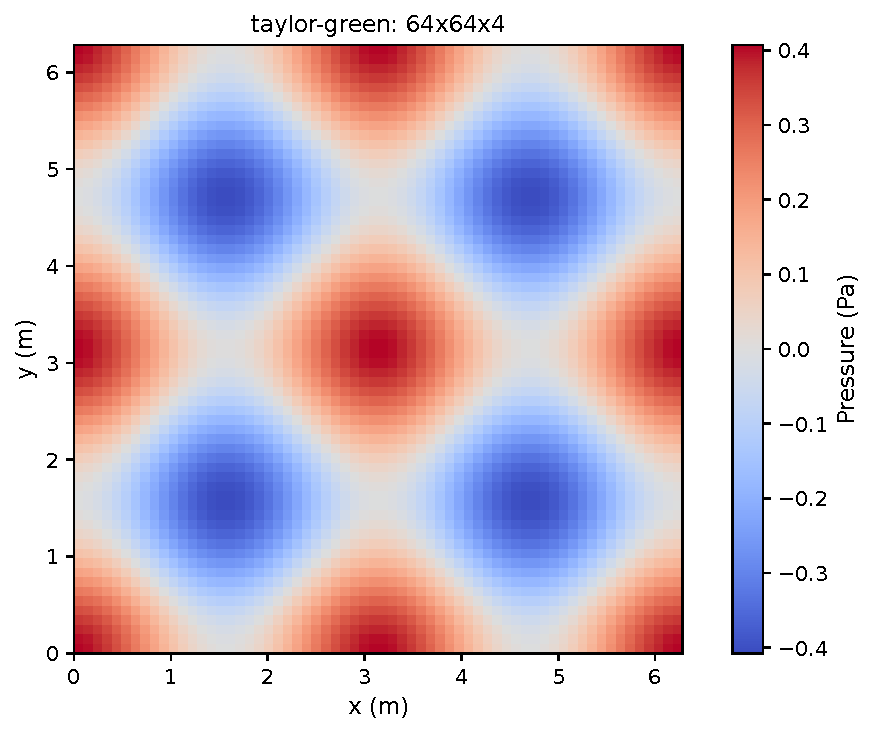
\includegraphics[width=0.9\linewidth]{tg-space-64/figures/pressure.pdf}\caption{taylor-green: pressure. Actual computed fields, SI units; comparison uses the documented reference region, gauge and time.}\end{figure}
\begin{figure}[htbp]\centering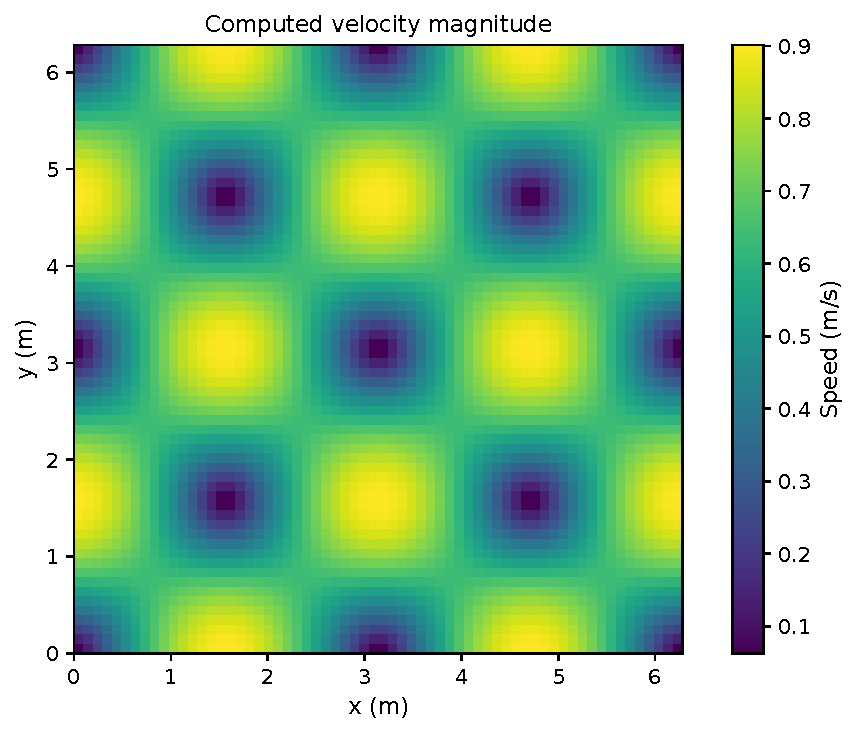
\includegraphics[width=0.9\linewidth]{tg-space-64/figures/speed.pdf}\caption{taylor-green: speed. Actual computed fields, SI units; comparison uses the documented reference region, gauge and time.}\end{figure}
\begin{figure}[htbp]\centering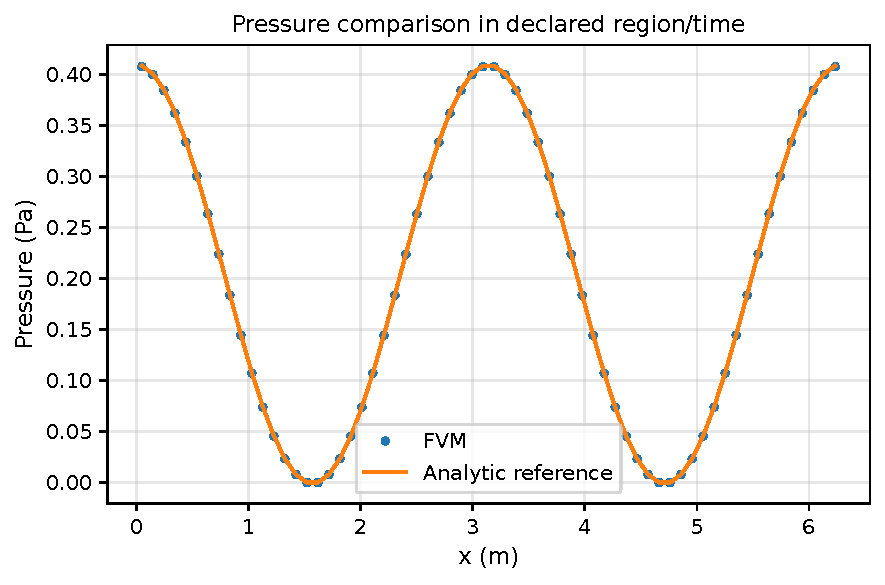
\includegraphics[width=0.9\linewidth]{tg-space-64/figures/pressure-curve.pdf}\caption{taylor-green: pressure-curve. Actual computed fields, SI units; comparison uses the documented reference region, gauge and time.}\end{figure}
\begin{figure}[htbp]\centering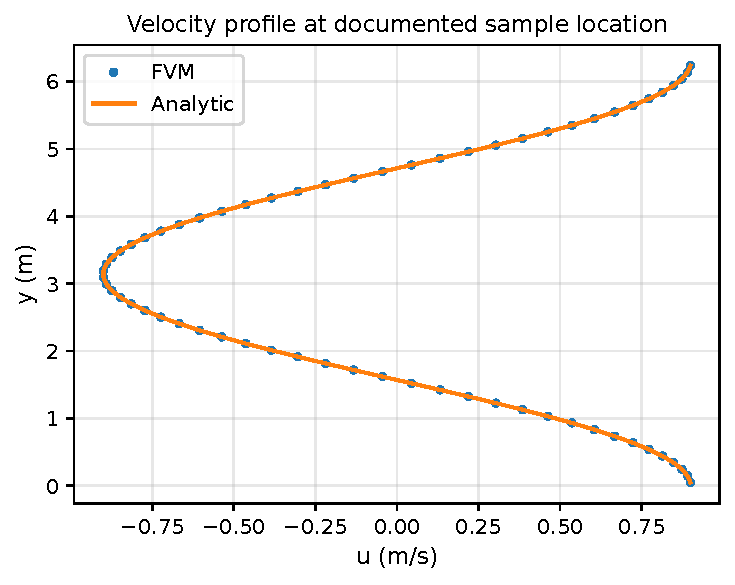
\includegraphics[width=0.9\linewidth]{tg-space-64/figures/velocity-profile.pdf}\caption{taylor-green: velocity-profile. Actual computed fields, SI units; comparison uses the documented reference region, gauge and time.}\end{figure}
\begin{figure}[htbp]\centering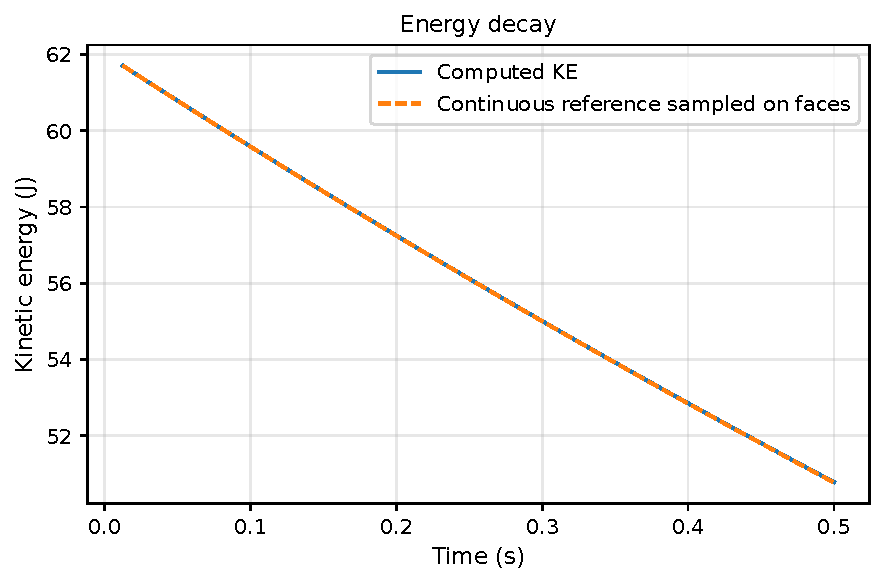
\includegraphics[width=0.9\linewidth]{tg-space-64/figures/history.pdf}\caption{taylor-green: history. Actual computed fields, SI units; comparison uses the documented reference region, gauge and time.}\end{figure}
\section{Matched TensorLBM comparison}
Both solvers use the same periodic continuum problem, SI parameters and end time. Errors use actual DOF locations and their respective pressure clocks. TensorLBM calls unmodified external D2Q9 BGK modules. The FVM advantages established here are incompressible pressure/face continuity, a discrete energy balance and time stepping independent of a lattice Mach mapping. Primary state storage per physical plane is four versus nine double arrays, not a peak-memory measurement. Different dimensions, step counts and diagnostic overhead prevent speed-superiority claims.
LBM 32x32: velocity L2 0.63348 percent, pressure L2 0.86173 percent. 
LBM 64x64: velocity L2 0.15207 percent, pressure L2 0.81428 percent. 
LBM 32x32: velocity L2 0.64003 percent, pressure L2 1.68311 percent. 
\begin{figure}[htbp]\centering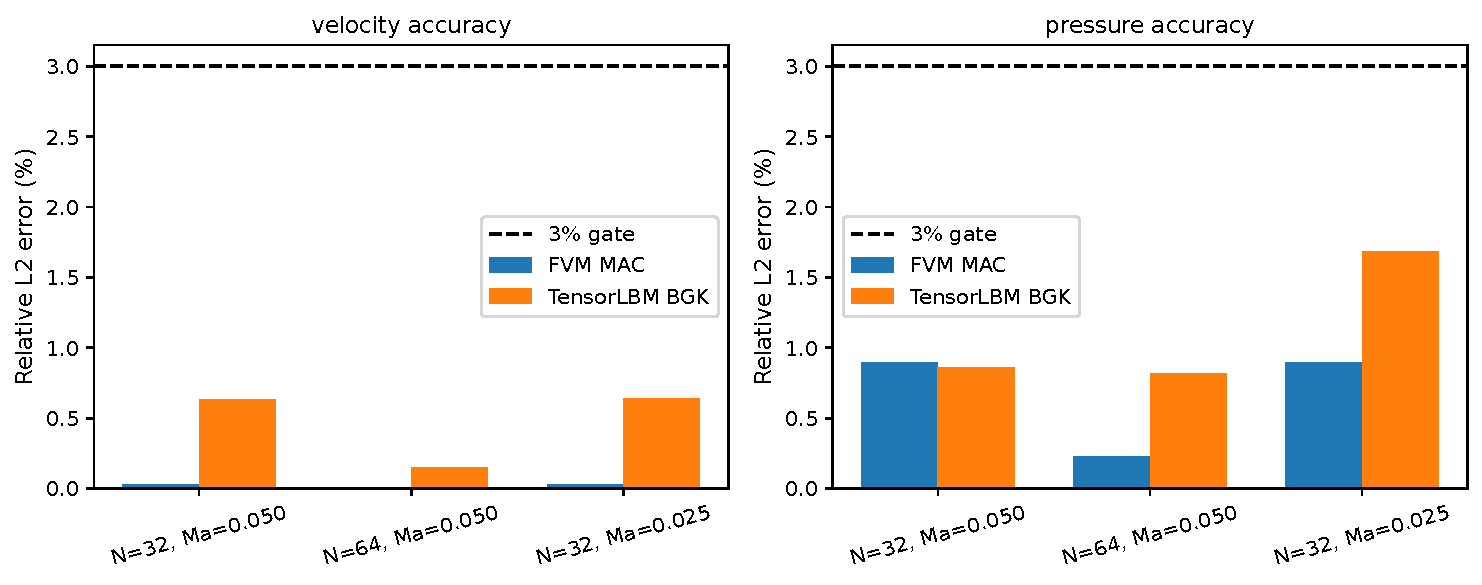
\includegraphics[width=\linewidth]{figures/fvm-lbm-errors.pdf}\caption{Matched analytic accuracy with declared Mach sensitivity.}\end{figure}
\section{Limitations and conclusion}
The vortex is a two-dimensional exact solution embedded in a three-dimensional mesh, not a turbulence benchmark. No qualification is claimed for free surfaces, moving bodies, ice fracture or coupled SUBOFF cases. The 3 percent criterion is a project target, not a universal publication standard. The analytic references follow directly by substitution into the governing equations. Negative controls are archived and excluded explicitly from regular-run qualification. A separate 128-square-grid run at dt=0.0125 failed its nonlinear solve; the retained failure must not be overwritten by the qualified 32/48/64 study. See the companion report and machine-readable summary for observed orders and all gate results.
\begin{thebibliography}{9}
\bibitem{tg} G. I. Taylor and A. E. Green, Mechanism of the production of small eddies from large ones, Proc. R. Soc. A 158 (1937), 499--521. DOI: 10.1098/rspa.1937.0036.
\bibitem{nasa} NASA NPARC Alliance, Examining Spatial (Grid) Convergence, \url{https://www.grc.nasa.gov/www/wind/valid/tutorial/spatconv.html}.
\end{thebibliography}
\end{document}
